\documentclass[12pt]{article}

\usepackage{graphicx}
\usepackage{amssymb}
\usepackage{url}
\usepackage[round]{natbib}
\usepackage[affil-it]{authblk}
\usepackage{color,hyperref}
\definecolor{darkblue}{rgb}{0.0,0.0,0.3}
\hypersetup{colorlinks,breaklinks,
            linkcolor=darkblue,urlcolor=darkblue,
            anchorcolor=darkblue,citecolor=darkblue}
\setlength{\parskip}{0.8mm}

\author{\sc{Daniel Arribas-Bel}}

\affil{
Department of Spatial Economics\\
VU University -- Amsterdam\\
\texttt{darribas@feweb.vu.nl}\\
\url{http://darribas.org} \\
}

\date{}

\begin{document}

\begin{titlepage}

\title{Accidental, Open and Everywhere: Emerging Data Sources for the
Understanding of Cities\footnote{This manuscript was prepared for the special session ``Urban Futures
2050'', held in August at the 2012 ERSA meeting in Bratislava (Slovakia) and
has been accepted for publication in \textit{Applied Geography}. 
%
The author would like to thank Julia Koschinsky, Ellen Schwaller and Emmanouil
Tranos for comments on a previous version of the paper. All the possible
errors remain the sole responsibility of the author.}}
%\maketitle


\begin{abstract}
In this paper, I review the recent emergence of three groups of data sources and
assess some of the opportunities and challenges they pose for the
understanding of cities, particularly in the context of the Regional Science
and urban research agenda. 
These are data collected from mobile
sensors carried by individuals, data derived from businesses moving their
activity online and government data released in an open format.
Although very different from each other, they are all becoming available as
a side-effect since they were created with different purposes but their degree
of popularity, pervasiveness and ease of access is turning them into
interesting alternatives for researchers. Existing projects and initiatives
that conform to each class are
featured as illustrative examples of these new potential sources of knowledge.


\end{abstract}

\paragraph{Keywords}
Data sources, Open data, Cities


\end{titlepage}

% \linenumbers

%% main text
\section{Introduction}
%Exciting time
These are exciting times to be an urban scientist. Not only is the world as a
whole becoming more and more urbanized, once the historical threshold of more
people living in cities than in rural areas has been already surpased
\citep{wup2007highlights}, but the ability we are gaining to look into the
inner workings of urban systems grows at even faster rates
\citep{batty2012smart}.
%Life more digital
An increasing amount of aspects of human life can be traced back through
diverse digital footprints and, when aggregated, can reveal emerging patterns.
%More of the economy is digital
Many economic transactions which used to be done
\emph{offline} have now been moved into the web, and their archival has created,
as a ``side-effect'', incredible amounts of data that reflect many aspects of
human behaviour.
%governments
Democratic governments have not been completely foreign to
technological change either. Many local, regional, national and supra-national public
institutions are moving parts of their infrastructure into the cyberspace and responding to
the presure of activists that demand more transparency by
releasing some of those data in open formats.
%
All of these recent societal changes did not explicitly intend to redefine the
``data landscape'' available to urban researchers, but they have, making
possible analysis at degrees of detail and scope unthinkable only a few years
ago.
% Ref. #1 comment
The traditional creativitiy that applied researchers (geographers,
economists, etc.) have developed to measure and quantify urban phenomena in
contexts where data were scarce is being given a whole new field of action. 
%

%What they share
The amount and diversity of new data sources relating to cities that is
becoming available grows exponentially\footnote{As a notable sign of this
increase in the amount of urban data and subsequent research, the
long-standing journal \emph{Cities} has created a meta-journal,
\emph{Current Research on Cities (CRoC)}, with the aim of summarizing the
field and pointing out current concepts in urban research.}, to the point it may seem
unrealistic to look at all of them as one entity. 
   %At first sight, tweets and real
   %estate prices aggregated from websites like Trulia, or Foursquare checkin's
   %and local public transit data do not have much in common, other than the
   %digital footprint they are reflected in. 
%
However, this paper argues that much of them share three key characteristics
that make them particularly well suited to current urban research. These
include:
their accidental nature, their open availability to
researchers, and the ubiquity of their presence in everyday urban life.
    %Accidental
First, unlike a census or an economic survey, specifically created
with research and policy analysis in mind, these sources were not originally
intended for this end but for other purposes. Its potential usefulness for
scientists comes then \emph{accidentally}, as a byproduct.
%
%   This is not without flaws and challenges, of course, but it also implies
%   clear advantages. Above all is their marginal cost: since most of the
%   resources needed to create them are justified by their primary use, the
%   additional burden required to generate useful datasets often comes in the form
%   of time and expertise (to store and tailor the
%   data).    
    % Open
Second, and partly related to the previous one, all of these sources
are available to researchers without the
need to pay any fee or reach exclusive deals with the company/institution
providing them.
    % Everywhere
Finally, given the degrees of pervasiveness
that are reaching the technologies and services where they originate, new
datasets relating to virtually any quantifiable aspect of human life are appearing.
% great opportunity
Similar to other fields (e.g. see \citealp{edelman2012jep} and
\citealp{einav2013bigdata} for recent reviews in the
case of economics), the combination of these three factors creates a
significant opportunity for urban and regional scientists to study
new phenomena or to examine old questions with a new insight.
%
Very much in line with the views of \cite{overman2010gis} in relation to
Geographic Information Systems (GIS), these data can in turn help: reduce location measurement error
of observations (although they may introduce other biases, see Section
\ref{challenges}); avoid the issue of discretizing continuous problems; fill
gaps where traditional data are unlikely to exist; and design
instrumentation strategies as a source of exogenous variation.

%In this paper, these new developments are categorized in three main groups
The main line of argument is that most of these data sources fall
into one of three main groups, based on the basic actor and the nature of
the process at which they originate.
%1 bottom-up
The first category is comprised by data collected in a \emph{bottom-up}
approach from mobile sensors carried by humans.
%2 meso-collector
At an \emph{intermediate} level, we can identify databases employed to provide
a (usually free) service through the internet by web companies. These are
typically aggregated from several primary sources and derive from businesses
which either move or base their activity on the internet.
%3 top-down
The last group is characterized by the \emph{top-down} fashion in which it is
collected, and it has to do with data released in an open format by public and
government organizations at different geographical levels.
%
This classification is not exclusive and may be combined with other ones as
well as inter-mixed (e.g. open govenrment data collected from mobile sensors,
as in what is become known as ``civic apps''). It is based on the intrinsic nature of the data origins
and, although simple, it can be powerful to better interpret their attributes and,
particularly, the type of processes or phenomena they may be reflecting.
Ultimately, it is the good understanding of what the data can and cannot
``tell'' that makes it possible to incorporate them into meaningful studies.

%Challenges
Although potentially very advantageous, the use of these data is not free of
challenges. Most of them derive from their \emph{accidental} nature, from the
fact they were not originally intended for this use. 
%Quality: completenes and bias
In particular, the major flaw may relate to the quality of the data: depending on what it is
that we are trying to measure, the degree of completeness and bias in the
population samples can compromise results and lead to misleading conclusions.
%Programming skills
But those are not the only hurdles to be confronted. Because often times they
were not intended to be used in bulk, collection can be tricky and require
some programming and database skills to access the sources.
%New methods and visualization
Once collected, the characteristics of the data may require methodologies and
techniques not very familiar to the field yet. In some cases, as
in what is come to be known as ``big data'', the size and lack of structure of the
datasets is such that applying traditional techniques may not be the preferred
solution and other methods, such as machine learning
\citep{Bishop:2006:PRM:1162264} or knowledge discovery
from databases (KDD) techniques \citep{JORS:JORS641}, as well as advanced
visualizations \citep{cheshireattyepb2012}, may prove more fruitful.
%
Section \ref{challenges} will discuss these issues more in detail.

%What this paper is not about
When dealing with such a broad topic, it is almost as useful to explicitly state what
\emph{is not} included as much as it is to describe what \emph{is} covered.
It is important to make clear that the main aim of this paper is
neither of the following.
%Not all the literature on that
First, it does not intend to be an exhaustive survey of all the 
literature that has already taken advantage of these new kind of data.
Although not vast (yet), the amount of publications using any of these three
sources is large and sparse enough that any attempt would be incomplete. Instead, I provide
a few illustrative projects as an example of the advantages to be benefitted
from and challenges to be assumed.
%Not about all new data sources
Second, this piece is not about \emph{any} possible new source of data that is
becoming available through the web or from public governments. The three
categories in which the data sources featured are conceptualized are fairly
broad and do include many of the new kinds of data appearing nowadays; however
there exist alternative ones that are not best conceptualized into either of the three
labels proposed in this work\footnote{For instance, although closely related,
\emph{volunteered geographic information} (VGI, see \citealp{goodchild2007vgi}
or \citealp{wikfication}) systems are not
explicitly covered in this context.}.
%Not about these data sources in any context (only on regional science/urban
%research)
Third, this will not deal with opportunities arising from the use of these
data in contexts other than academic research in the fields of urban and
regional science. 
This is not to say those are nonexistent or irrelevant; on the contrary,
applications in other fields can be highly benefitial,
both in private (e.g. geo-targetted marketing) and social (e.g. disaster
management, social services efficiency) terms.
However, the strength of this paper is on bringing into the attention
of those two academic communities these new advances in
the hope it will ease their adoption for
future research and, as such, it will be confined to that specific end.

This paper takes a practical approach by
exposing the nature of these data sources in an accessible way. This is done
purposely to reach as many potentially concerned regional and urban
researchers as possible and stir their interest.
% Ontological essay
For the advanced reader, a more explicit treatment of ontological and epistemological aspects of the
use of this kind of data can be found in \cite{warfsui2010},
\cite{boydcrawford2012} or \cite{crampton2013geotag}.
% Political economy
Equally important aspects such as its political economy or issues
underlying their production can be found in \cite{leszczynski2012} or in a
recently compiled edition by Lisa Gitelman \citep{gitelman2013oxymoron}.
%
The rest of the text is structured as follows: Sections \ref{sensors} to
\ref{gov} describe the emergence and characteristics of the three
different categories mentioned above, suggest how they can be helpful for
researchers interested in urban issues and feature projects and iniciatives led by
different actors that serve as real illustrations; Section \ref{challenges}
discusses some of the challenges that these new data sources pose when
contrasted with the ones traditionally used by the social sciences; and
Section \ref{conclusions} concludes with a few remarks and highlights.

\section{``Citizens as sensors'': collecting data from the bottom-up}
\label{sensors}
%Emergence
%Technology is following us everywhere. This statement, probably appropriate
%for the humankind ever since the beginning of civilization, is
%currently reaching its most literal implications.
%Internet --> smart-phones
The invention of the internet and its ubiquitous presence nowadays,
particularly reinforced with the emergence of mobile
devices\footnote{According to a recent study \citep{msInternetUsage2012}, the
number of mobile users of the internet is expected to exceed that of desktop
users before 2015.} such as smartphones
and tablets, has created a platform in which every aspect of life is subject
to leave a digital trace.
%Examples: blog post, uploaded picture, tweet
Not only obvious ones like internet behaviour (browsing patterns) or economic
activity (in the form of online purchases for instance), but also more traditionally
intimate aspects of humans are being stored online: opinions are reported in
blog posts, memories in pictures uploaded to social networks and even feelings
or moods may be reflected on micro-blogging services such as \cite{twitter}.
%citizens as sensors
When we conceptualize internet-enabled mobile devices as
extensions that empower human beings, \emph{citizens} effectively become
\emph{sensors} \citep{goodchild2007vgi} that produce streams of data that in
turn can help reveal different aspects of their own nature.

%Many ``freely'' available
This section is dedicated to a subset of these sources particularly promising due to
its ease of access: that freely and openly available on the web. 
Many of these data are broadcast by individuals directly to the internet and may be
accessed by other people (in fact that is usually the main aspiration of the ``data
producers'', to be reached). 
%API
Not only are they readily available but, in many cases, access is even encouraged by the
providers. As an example, many social networks, such as \cite{facebook} or \cite{twitter},
offer application programming interfaces (APIs) that allow developers to
access (part of) their data in an automated way. Although these APIs were
initially designed to build third party applications or services, their
existence opens up the door for researchers to access these
sources without having to reach any previous
agreement. This has a democratizing effect in that the potential set of
researchers that may access and work with the data expands beyond those able
to reach exclusive deals.

%Which ones they are. Characteristics
The speed at which new services and networks appear, gain popularity or
dissapear is such that any
effort to list or create a full inventory is not only hard but also becomes
useless quickly. However, it is possible to identify them by considering the following
three characteristics.
%
The defining attribute of this group, which also represents its main
advantage, is the micro-nature of the data: they originate and are
contributed at an individual level and, unlike 
the data sources covered in the next section, when they are accessed, this
characteristic is retained.
    %Web 2.0
    Second, their individual dimension also makes them part of what is come to be known as \emph{Web 2.0}, a
    concept that captures some of the changes in the internet industry that have turned
    end-users from mere content consumers into both consumers \textit{as well as}
    producers. This aspect is important because it is based on the generation of
    user content that most of the interesting databases are created.
    %Social component
    Third, they usually have embedded some sort of \emph{social} functionality
    that connects users and turns the experience from an individual one into a
    community based one. This feature is a more recent one and offers great
    opportunities for social network analysis.
    %individually created and uploaded data 
   %Third, the advantage of this group in terms of the type of data generated is
   %that they originate and are uploaded at the \emph{individual} level,
   %presenting thus a high degree of resolution and detail.
%
%Examples: facebook and ttwitter (more open)|particular ones: Flickr, RunKeeper
The main examples are \cite{facebook} or \cite{twitter}\footnote{The open
nature of this social network in which very few users effectively change their
settings to make their content private is probably at the heart of its success
and also the reason why it is one of the most evident candidates to use as data
for research.} but also more activity-focused ones such as Foursquare
(location sharing), Flickr (photography) or GoodReads (books).
%not mobile phone (cite botarziello + Tranos)
On the contrary, the condition of free availability effectively rules out other related sources that, due to
confidenciality, privacy or security issues, are not publicly available. A
particularly close and relevant case is that of mobile phone data. Although it also
originates in mobile devices, its access is restricted and, when available,
usually requires agreements with service providers. Its potential has
already been assessed and reviewed in studies like
\citealp{steenbruggenMobile2011}, for example.

%GPS --> urban lens
In the context of this paper, these phenomena become specially relevant when an
additional characteristic is taken into account: many of these digital traces
incorporate the geographical coordinates of the location where the
event occurs. This has been posible due to the popularization of
location-aware technologies such as the global positioning system (GPS)
and their inclusion in modern mobile devices. Such innovation has clear
implications for the nature of the data produced, which immediately gains a
spatial dimension. In fact, it is this possibility of connecting events with the
location where they occur that appears as the most attractive aspect for
urban and regional scientists.

%How they can be useful for Urban studies 
The combination of individual data that reflect different aspects of human
behaviour with the availability of spatial coordinates to geographically
locate such activity poses important opportunities to applied urban and
regional research.
%collected and accessed at the individual level
The individual nature has already been mentioned;
%Constantly updated
these data are not only highly detailed in space, but also in time. The large
volume generated by these sources and the high frequency with which
they are updated means they can be understood as a stream of data in real time
rather than as snapshots over periods. This represents a leap forward when
compared to the frequency at which other traditional sources are published
(e.g. ten years in the case of most censuses). It also has a remarkable
potential to inform models with intensive data requirements, such as time geography approaches
\`{a}-la-H\"{a}gerstrand as remarked in \cite{sui_hagerstrand}, or to bring
insight in situations where there is severe lack of traditional data but the
degree of pervasiveness for mobile technologies is large, such as
developing countries\footnote{As an illustration of the
potential in this realm, a team of researchers at IBM developed the project
``AllAboard'' \citep{allaboard2013} which implements a system based on mobile
phone data that optimizes the public transit network in Abidjan, the capital
of Ivory Coast.}.
%
This degree of detail and scope allows for a fresh approach that is likely to
bring new answers to traditional lognstanding
questions in the Regional Science and urban literatures, such as commuting or
aggomeration economies, for example.
In fact, the picture that best describes these
sources of data is that of an incredibly detailed lens through which to look at cities.
This new capability may represent a shift in urban research in
a way that, as \cite{lohrNYT2012} suggests, is akin to the invention of the microscope four
centuries ago.
%
%   At an academic level, such combination of detail insight about human behaviour with
%   accurate spatial reference may also help intensify the interaction between
%   \emph{economists} and \emph{geographers}, one that although not very deepened,
%   promises fruitful outcomes \citep{Rodrguez-Pose01032011}.

%Existing work outside Regional Science
Although very promising, the scientific use of data of this nature for urban
purposes is still at a very early stage. The first
explorations into its potentials do not come from traditional urban and regional
fields but from computer science researchers. The emerging field of
Computational Social Science \citep{compSocSci2009science} and, in particular,
that of ``urban computing'' \citep{cranshaw2012livehoods}, of
which good examples are \cite{calabrese2011connected}, \cite{Cranshaw:2010:BGP:1864349.1864380},
\cite{cheng2011checkins} or \cite{noulas2011}, is at the forefront. 
%
Mostly due to differences in traditions, backgrounds and interests, these
studies set an emphasis on the \emph{computing} side rather than on the \emph{urban} one. In
particular, this is reflected on a combination of expertise from computer
science and engineering to study cities.
%
In the next section, I cover in more detail one of its most prominent
illustrations as a case of use of this sources of data.

% Featured project: Livehoods
\subsection{The \emph{Livehoods} project}

\begin{figure}[<+t+>]
   \begin{center}
    %Figure \texttt{livehoods.png} approximately here (on top of page)
       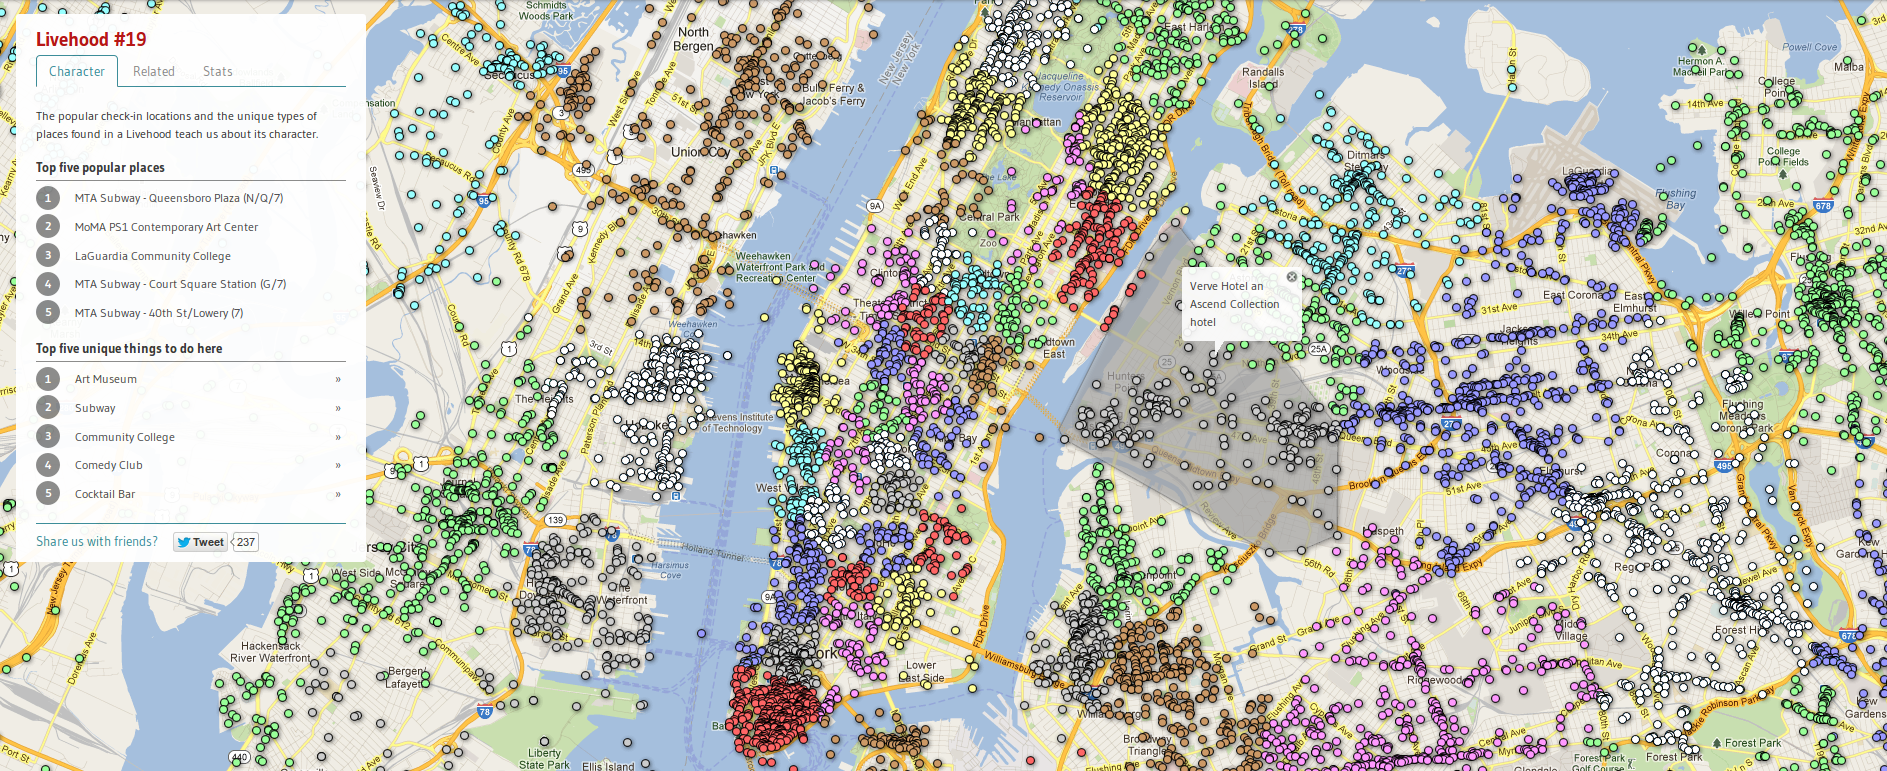
\includegraphics[width=1.0\textwidth]{livehoods.png}
   \end{center}
   \begin{footnotesize}
       Source: Screenshot captured from
       \url{http://livehoods.org/maps/nyc} on September 10th., 2012.
   \end{footnotesize}
   \caption{Example of \textit{livehood} in New York City}
   \label{fig:livehood}
\end{figure}
%% Overview
``(T)he 'character' of an urban area is defined not just by the types of
places found there, but also by the people that choose to make that area part
of their daily life'' \citep{cranshaw2012livehoods}. That is the main
motivation behind the Livehoods project
(\url{http://livehoods.org}).
%
The project aims at drawing the boundaries of what are called
\textit{livehoods}, areas of similar character within a city. Unlike static
administrative \textit{neighborhoods}, the \textit{livehoods}
re-define cities based on the habits of people who live there.

%% How they use this source of data
The delineation relies heavily on data from Foursquare, a location-sharing service
in which users can instantly broadcast their location from their smart
device in what is termed a \textit{checkin}. Leveraging a database of about 18
million checkin's of many users, the researchers use machine
learning techniques to cluster venues based on the users that frequent them.
Applying an explicit rule of geographic proximity, the result is the
livehoods: subsets of a city whose establishments (restaurants, bars, bookstores, stations,
etc.) have a similar clientele or, in other words, where people who go to one
of their venues also go very often to the other ones.

%% How is instructive + lessons that can be learned
The project is a good example of use of the data sources covered in this
section to increase our understanding of cities. Neighborhood delineation has
been a challenge for urban social sciences (see, for example,
\citealp{rey2011dynamics}).
Taking adavantage of the fine
spatial and temporal granularity, as well as its ready availability
online (the entire database was scraped from public posts pushed to
tweets), the researchers are able to obtain urban pictures
that would not be feasible with traditional methods such as surveys, and to gain
insight on how the social component can be measured and captured providing, in
this case, a different view on the neighborhood construct than it was
available before.
% Only one example
This is however only one among many other possible uses that urban
scientists could find for these kind of data. Alternatively, the project is a
good case to hint at how the output of its analysis could be incorporated in other
studies. For instance, once constructred, the livehoods could be used as the main units of
analysis, in an effort to capture the most accurate unit of analysis and avoid
the so-called modifiable areal unit problem (MAUP,
\citealp{openshaw1981modifiable}).

\section{Businesses moving online (and creating data in the process)}
\label{web}
%Intro
Not only individuals' lives are moving online, companies are also hopping on
the internet train. 
%%Traditional offline businesses moving online (Trulia)
In certain sectors, the popularization of the web has created important challenges but
also opportunities to the traditional business model. Some firms have embraced
them and have significantly increased their productivity and efficiency.
Although this technology has been inserted in many diverse ways at different stages of
the production chain, its inclusion as an additional factor has
always been reflected in an increase of digital
data about the economic activity undertaken.
%
In some cases, these data are
also exposed to the general public, creating an opportunity for
researchers as well. As an example, the real state
market has witnessed a transformation in recent years that has greatly
improved the availability of information. Consumers nowadays have free access
to online databases provided by websites like \cite{zillow}
or \cite{trulia} that aggregate data from local
brokers, providing a much larger overview of the market as well as additional
information merged from diverse sources. These data are usually freely
available via websites or machine readable APIs, which facilitate
their extraction.
%%New online natives (WalkScore)
In addition to online companies covering offline businesses, there
has also been an outburst of \textit{internet natives} covering new portions
of the market. These firms do not have a clear offline counterpart and they
are usually data intensive, meaning (digital) data are a key part of their
business model.
%Open Availability in many cases
Because many of these sites offer their services free of charge (the revenue
is collected through advertising or other means), much of the data are
available to researchers as well.
% Ref 2. comment
This aspect is key because it sets the sources reviewed in this section apart
from more traditional data-oriented companies. There is a
long-standing tradition of firms whose main business model is to collect and
\textit{sell} datasets to researchers or analysts
(e.g. ESRI's Business Analyst establishments database or Experian's real state
datasets). Although very relevant in some contexts, where their contribution has not
only been useful in itself but also in creating synergies with the public
sector and in influencing public data collection, their ``non-accidental''
nature leaves them out of the main focus of this paper.

%Main characteristics
%%Aggregates
The spatial as well as temporal availability of these sources of data is much
more diverse than for those in Section \ref{sensors}. Fine granularity may be
found in either time (e.g. \citealp{trulia}) or space (e.g.
\citealp{walkscore}), but rarely in both.
%%Less time resolution but still usually better than Census
Although, in most cases, the data is not released in ``real-time'' but
aggregated at some sort of scale, the periodicity at which they can be
obtained is usually better than that of official sources such as census
bureaus, which makes them very attractive for studies in which the interest
lays in the temporal evolution of some sort of urban phenomenon.
%%Non-usual topics --> Link to next paragraph
The biggest advantage of this family of sources is the large variety of
aspects they can cover: because they originate from the most diverse
businesses and range of economic activities, they have the potential to
provide measurement on aspects of the economy that used to be unimaginable to
capture in data. 
%Complement/supplement of traditional sources (Census, ACS)
   %The relation with more common datasets, such as censuses or public surveys
   %like the American Community Survey (ACS) does not have to be mutually
   %exclusive. On the contrary, both types can be combined to enrich each other's
   %weaknesses. As an example, events can be aggregated
This better periodicity and sometimes more detail should not be seen as a
reason to understand this group of sources as a
replacement or substitute of more established ones such as censuses or
national surveys. On the contraty, it should be considered as a complement, an
alternative that may fill particular needs or that may be merged to
more traditional datasets in order to capture the process of interest.

%More has been done in Regional Science: Feldman's iniciative
Unlike data of more recent nature, these sources have already been included in some studies
within the urban and regional science fields (e.g.
\citealp{avnimelech2011impact}) and have proven successful in bringing
empirical insight on aspects that traditional data did not allow to capture or
identify. Moreover, recent iniciatives such as
\cite{feldman2012data}, ensure that in the future only more studies will take
advantage of their properties. As an example of these sources, the next
subsection presents Walk Score, and online company which produces an index of
walkability.

%Featured project: WalkScore
\subsection{WalkScore.com}

\begin{figure}[<+t+>]
   \begin{center}
    %Figure \texttt{walkscore.png} approximately here (on top of page)
       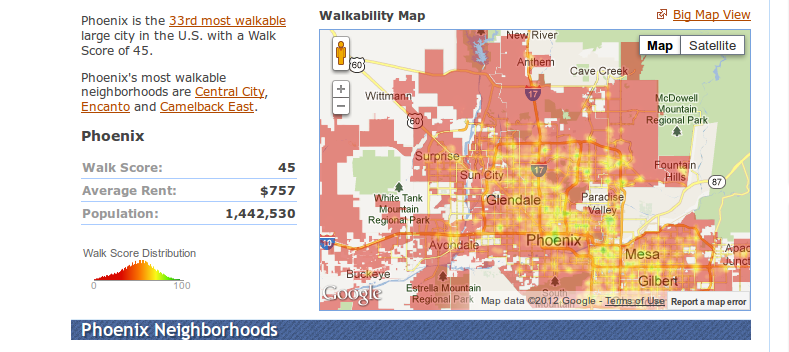
\includegraphics[width=1.0\textwidth]{walkscore.png}
   \end{center}
   \begin{footnotesize}
       Source: Screenshot captured from
       \url{http://www.walkscore.com/AZ/Phoenix} on September 10th., 2012.
   \end{footnotesize}
   \caption{Surface of Walk Score for Phoenix}
   \label{fig:livehood}
\end{figure}

\cite{walkscore} was originally a project of Seattle-based company
\cite{frontseat}. Its purpose is ``to promote walkable neighborhoods'' and,
ultimately, their aim is for walkability to be included as a typical
characteristic of a house (as their website says: ``Our vision is for every
property listing to read: Beds: 3 Baths: 2 Walk Score: 84''). In essence, the
walk score (WS) is an index that factors in several aspects of walkability
such as accessibility and street network characteristics to offer an overall
measure of the walkability of a location, as defined by its latitude and
longitude coordinates. The data are freely available on their website as well
as through an API and may be collected for every point within the set of
covered cities\footnote{See \cite{walkscoreWhite} for a detailed
description of the methodology and
\url{http://www.walkscore.com/rankings/cities/} for a list of US cities for
which WSs are provided (last accessed: September 5th., 2012).}.

Currently, WS is mostly used by real state brokers and realtors to capitalize
on the value of walkability. However, the index is slowly permeating in
empirical academic research as well.
% Validation
Some of them (e.g. \citealp{duncanWS2011} or \citealp{car2010ws}) have first focused on
validating their use vis-a-vis more traditional measures, finding very positive results;
% Application
while others have used the index in applications on fields as diverse as real
state (e.g. \citealp{locationmortgage2010JORSE} and \citealp{pivo2011ws})
or urban design (e.g. \citealp{emilyjulia2013}).
%
Scholars are starting to use it to
replace traditional measures, which usually require a larger time and
financial investment to collect. This is opening up the door to carry out
studies on walkability at levels that were not feasible a few years ago.
%
As an example of large scale analysis, WS has recently been included in
a project that aims to evaluate walkability and its relationship with
affordable housing at the US national level \citep{kochinskyTalen2012hud}.

\section{Open Governments, open data}
\label{gov}
%Intro and why
Opposite to data in Section \ref{sensors}, the last family of sources is the
reflection of a ``top-down'' process, in which public
organizations release some of their internal data in open format.
%Higher transparency and efficiency
In effect, governmental organizations, from the national
level down to local
authorities, are making available increasing parts of the data they collect
while developing their activities. 
%% Four reasons
This process if fueled mainly by four main strategic drivers
\citep{datagovukslides}: transparency and accountability, economic and social
value, public service improvement and creation of new industries and jobs.
%% Transparency (data journalism)
The first one is a response to citizen demands and may be seen as a tool to build trust
\citep{opendatawp}. By allowing external parties to access,
review and study internal data, it becomes easier to identify and attribute
responsibilities in cases of, for instance, corruption. Closely related to this
goal is the emerging field of ``data journalism'' (\citealp{sacredfacts},
\citealp{djhb2012}), which has played a role in the development of open
government data and is based on the idea that data, just like text or photographs, can be
a powerful tool to inform and hold governments accountable
in cases where needed, hence collaborating to the function of 
press in a democratic society.
%% Budgets and Efficiency (Gov 2.0)
On the other hand, there is a more pragmatic reason as well that oversees the
last three main drivers. The opening of data can be a succesful strategy not
only to serve the democratic goals of a government but to turn
it into a more efficient and impacting organization. This has been
pointed out by the so called ``Government 2.0'' movement, which aims at
improving the effectiveness of governments by the introduction of
technology and practices borrowed from the computer world in their processes.
As \cite{govplatform2010} puts it: ``Government 2.0, then, is the use of
technology -especially the collaborative technologies at the heart of Web
2.0- to better solve collective problems at a city, state, national, and
international level''.

%Very diverse data in nature and topics
At the moment of writing, \url{http://data.gov.uk} (UK) exposes 8,680 datasets and
\url{http://data.gov} (US), 378,529 raw and geospatial datasets, and those are only two
of the main government portals. This vast amount of
data is as large in quantity as it is in diversity. A quick browse through the
index reveals items as disparate as ``US DOE/NNSA Response to 2011 Fukushima
Incident: Radiological Air
Samples''\footnote{\url{https://explore.data.gov/Geography-and-Environment/US-DOE-NNSA-Response-to-2011-Fukushima-Incident-Ra/u9mw-zn8r}}
and ``Central Contractor Registration (CCR)
FOIA''\footnote{\url{https://explore.data.gov/Information-and-Communications/Central-Contractor-Registration-CCR-FOIA-Extract/3hqn-qzh6}}.
%New opportunities to analyze data
Clearly, not all of this is potentially relevant for urban and regional
research. However there are still reasons to consider these
sources. Many of the data have location information and can hence be
geographically pinpointed, which provides them with a regional dimension.
In addition,
the incredible diversity and abundance of data in these portals, makes them a
good archive when looking for proxy variables of phenomena for which
data are not at hand or sources of exogenous
variation within an identification strategy, for example.

%Regional and local data
The wave of opening data does not stop at the national level.
Many regional agencies and local administrations are joining this trend as
well.
Cities like New York (\url{https://data.cityofnewyork.us}), Chicago
(\url{https://data.cityofchicago.org}) or Paris
(\url{http://opendata.paris.fr}) have started open data portals in which they
upload datasets about many diverse aspects of the city. As an example of clear
interest for urban researchers, next is considered the iniciative of the
Metropolitan Transportation Authority of New York City.

\subsection{MTA transit data}
% Featured project: MTA transit data

\begin{figure}[<+t+>]
   \begin{center}
    %Figure \texttt{nyc.png} approximately here (on top of page)
       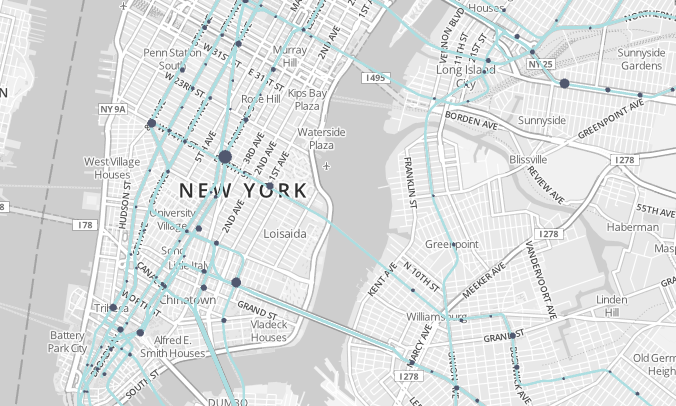
\includegraphics[width=1.0\textwidth]{nyc.png}
   \end{center}
   \begin{footnotesize}
       Source: Screenshot captured from
       \url{http://data.fabernovel.com/nyc-subway/} on September 17th., 2012.
   \end{footnotesize}
   \caption{NYC Transit System}
   \label{fig:nyc}
\end{figure}

In 2010, the Metropolitan Transport Authority
announced the release of part of the data about the public
transit system in New York City in an open format \citep{mtaopen}.
% What kind of data is released
Basically, this includes service and schedule data as well as other
characteristics of the transit system such as hourly volume of \emph{swap-in}'s and
\emph{swap-out}'s in subway stations.
% What is the original purpose
In this case, the original purpose is to put the data out so some services can
be outsourced at low cost, increasing thus efficiency in the provision (``make data available to software developers who
are interested in creating smartphone or web applications -- or ''apps`` --
that help our customers'').
% What can it serve to the urban researcher
However, free access to this kind of data represents a tremendous opportunity
that used to be restricted to the few researchers that were able to reach
agreements with the agency.
%% PArticular MTA dataset
    %More than one in two New Yorkers (55\%) commute by public transit (2010 ACS
    %5-year estimates)
    %http://factfinder2.census.gov/faces/tableservices/jsf/pages/productview.xhtml?pid=ACS_10_5YR_B08101&prodType=table
More than one in two New Yorkers (55\%) commute by public transit
\citep{acs2010-5year_est}. Having direct access to data that describes and
characterizes this phenomenon at such refined scale certainly makes possible 
interesting analysis for transport engineers, urban economists and planners.

%% More general lesson
The MTA iniciative is only one example of a more general trend that is
perhaps best exemplified in the public transit case\footnote{For a detailed list of
municipalities offering transit data in open format, see
\url{http://code.google.com/p/googletransitdatafeed/wiki/PublicFeeds}.} but
that spans a much larger case scenario. From local finance data to urban tree
canopy metrics, the
release of open public data has the posibility to positively impact much of
the applied research conducted about cities and regions by allowing access to
previously restricted data to a much wider scientific community.

\section{Challenges}
\label{challenges}
So far, this paper has stressed only the benefits of these new sources of
data. The reader up to this point would be tempted to wonder why, other than
their novelty, they have not been used more intensively in urban research. 
One of the most obvious answers is that they, as many other types of data
typicallly used, also have some drawbacks and imperfections that may prevent
their use in some contexts.
%
In order to obtain a full picture of the characteristics and nature of the
data reviewed above, this section presents three main obstacles that pose
challenges for their direct application in scientific research about
cities\footnote{For a more complete review of challenges to the new age of
large datasets in social sciences, see \cite{king_science_ensuring}.}.
The first one relates to the quality of the data, the second to the set of
skills required to take advantage of these databases and the third one
reflects on the suitability of traditional methods that were meant for
traditional data. 
% Privacy and ethics
In addition to these, issues about governance and
ethical questions are becoming of greater concern, particularly as it is
becoming clear that it is very difficult to maintain privacy even in
anonimized datasets (e.g. see \citealp{unique_crowd} for the case of cell-phone
data). Although very relevant, these
aspects are not directly related to the adoption in research of the data
sources reviewed and, consequently, are left out of
the paper. The interested reader
can find a more extensive treatment in the literature on smart cities, of which
a good recent overview is \cite{battyetal2012smartcities} or \cite{kitchin2013}.

%Quality: completeness and bias
One of the most prominent preocupations when trying to understand phenomena
through data is to what extent the sample is representative of the population
of interest. This is of particular concern when it comes to data that, for the
most part, requires very
particular characteristics in the user for it to be generated (e.g. to own a
smartphone), to the point of posing deeper questions on the
conceptualization of the world online \citep{grahamzook2013augmented}. The extent to which
this is a problem depends of course on both
the exact type and source of data as well as the particular question being
analyzed. While some of the sources reviewed in this context could raise
issues of representability (e.g. Foursquare data as a representation of the
preferences of a whole population), others do not suffer from that problem
(e.g. MTA data on subway usage as a representation of subway usage
in NYC).
%% in some cases the bias is as desired
In addition, there are two more reasons to be positive about the use of these
data. First, the increasing degree of penetration that the technologies powering
these data are reaching can only improve the current situation.
Second, in some cases the bias introduced by the data runs in a positive
direction. As an example, \cite{urbanity_photo2012} discusses how the
overrepresentation of young highly skilled professionals in
the users of photo-sharing services such as Flickr or Picasa can in fact
favour the analysis of the influence of urbanity in housing prices by
better capturing the preferences of the segment of population that is a potential
buyer of houses located in attractive areas.
%% In any case, something to take into account but to use to ditch the data completely
In any case, although present and potentially important, the existence of
quality and representability issues in these new sources of data should only
be one more characteristic to take into account and properly deal with but not
a total deterrent that precludes its use in contexts where it is sensible.

%Skill set as an entry barrier
A more subtle underlying cause of the lack of research using
open web data is the different barriers to access them in raw
format. Many of these sources are exposed to the
world through APIs or in a form that require some pre-processing before
becoming tabular data (e.g. raw text or html). 
%% Referee 1 comment- structured Vs. Unstructured | relational Vs. No relational
%   This is particularly true in the case of unstructured large datasets, where
%   no pre-defined or tabular structure of the data is known,
%   since the need of expertise on particular tools such as non-relational
%   databases of natural language processing techniques is even more acute.
%%APIs and programming
The interested researcher then needs to have some basic
general programming skills that allow him or her to write simple scripts to
query the database, usually over the internet. Although this is not a
particularly difficult task, it is certainly more intricate than a simple bulk
download from a data portal, as most researchers are used to when it comes to
obtaining more traditional data. The relevance of this aspect however, is also
bound to diminish over time. As computational methods and larger datasets
increase in importance and amount in social science research, the returns to learning basic
programming capabilities and aquiring expertise on databases other
than the traditional data sheets will increase. In fact, it is possible that eventually,
they become part of the standard set of tools an applied quantitative social researcher is
required to master in order to qualify as such, similar to the way typesetting
systems (e.g. \LaTeX  or Microsoft Word) and statistical packages
(e.g. Stata, Matlab or R) are nowadays.

%New methods for new data: Data Science
Finally, there is also a case to be made about the suitability of the current
methods to analyze and obtain insight out of the databases arising from some
of these new sources. 
%
Many of the statistical techniques in use in regional
science and urban analysis nowadays were created
in a context in which data were characterized for its limited availability rather than for its
over-abundance. 
    %This implies that many methodologies were designed with
    %scarcity of data in mind and thus tend to impose some sort of ex-ante structure in order to
    %produce sensible results.
%
This paradigm might be shifting and, if that is the case, new methods to complement the
existing ones will be required. 
%
As \cite{skupinAgarwal2007} mention in the context of large georreferenced
datasets, ``traditional inference methods are either
failing or have become obstacles in the search for geographic structures,
relationships, and meaning'' (Ch. 1).
%
Such new generation of modelling techniques
will have to expect continuous rather than discrete, large rather than small
and, in some cases, real-time rather than delayed data.
%
This will translate into a family of analytics in which the
assumptions about the structure of the data will be traded for the ability to
be applied fast and at a large scale.
% Ref. #1 comment on analytics
In some cases, as it happens with monitoring systems as those reviewed
in \cite{kitchin2013}, the approach will have to be revisited not only in
terms of the algorithms used but also in relation to the data infrastructure required to
support real-time analysis based on a continuous stream of data.
%
The response from the industry to this phenomenon has been the new and emerging field of
``data science'', a blend of statistics, engineering and computer science
that aims at creating value from the streams of data generated by the online
economy\footnote{\citealp{mgi2012bigdata} review its emergence and particularly note the
shortage of properly trained labor force in comparison to the existing and
future demand}. 
% More borrowing from DS
If more of these types of data are to be included in regional and urban
studies, researchers will also have to embrace these techniques in
order to exploit all the meaninful information,
and ``borrowing'' from fields like machine learning or information
visualization, for example, will have to become a more common practice than it
is nowadays.

\section{Concluding remarks}
\label{conclusions}
% What it's done
This paper has reviewed the emergence of three new sources of data that
may be useful for the regional and urban scientific communities. These are
data coming from individuals carrying location-aware devices, from businesses
moving (some of) their activity online and from governments releasing
an increasing share of
their data in open formats. For each source, a detailed characterization has
been given as well as a real world case that serves as an example. A
particular focus has been set on the subset of these sources that may be openly and freely
accessed by researchers. The overview is complemented with a set of challenges
posed by their nature and characteristics that are precluding its ready use in
applied urban research.
 
Ultimately, these new data have the potential to bring new answers to old
longstanding questions in the different fields of urban analysis, and that has
been the main premise behind the motivation of this paper.
%
The ability to look at urban phenomena through the potentially much more
detailed and granular lens these data allow for should be put at the service
of existing theoretical premises.
% Inter-disciplinary glue
However, given the particular characteristics outlined in the previous
sections, these sources of data can also be a positive force towards higher
integration between disciplines. In fact, they could be seen as a sort
of interdisciplinary ``glue'' that favours
cross-pollinization between fields where such interaction has been coming for a long
time (e.g. economics and geography, \citealp{Rodrguez-Pose01032011}) or that
induces new creative collaborations within the Humanities as suggested in
\cite{delyserSui2012phg}.
%
Equally, the popularization of such data is likely to also
strengthen the linkages between GIS and spatial analysis noted in
\cite{goodchildHaining2004}.
%% Ref-2 comment about making available 
Related to interdisciplinarity is the question of data
availability and transparency in science. Although not exclusive to the sorts of data
reviewed in this text, the tremendous increase in the volume and variety of
origins and quality these sources are bringing with them calls for a policy of
transparency and, when possible (i.e. when not
limited by terms of use or licensing issues on the data providers' end), of
reproducibility \citep{peng2011science}\footnote{In this regard, it is
remarkable the new open access journal \emph{Sientific Data}
(\url{http://www.nature.com/scientificdata/}), whose mission is to publish
descriptions of scientifically valuable datasets.}.

%Main purpose
Rather than claiming discovery or exhaustiveness, the main purpose of the
paper is to bring the attention of researchers who are actively conducting
regional and urban analysis to the existence, availability and usefulness of
these sources as a complementary alternative to those already in wide use
(such as population censuses or surveys). In that sense, it should not be
viewed as a plea to completely replace the existing data used in the field
but, rather, to incorporate these new ones and to
develop strategies to combine the best of both worlds in search of new insights.
%
In an increasingly complex world, we need every possible tool
at hand to understand it and be able to deal with the problems of the new Century.
%
There is a new microscope available, it is now up to the researcher to use it.

% References


%% The Appendices part is started with the command \appendix;
%% appendix sections are then done as normal sections
%% \appendix

%% \section{}
%% \label{}

%% References
%%
%% Following citation commands can be used in the body text:
%%
%%  \citet{key}  ==>>  Jones et al. (1990)
%%  \citep{key}  ==>>  (Jones et al., 1990)
%%
%% Multiple citations as normal:
%% \citep{key1,key2}         ==>> (Jones et al., 1990; Smith, 1989)
%%                            or  (Jones et al., 1990, 1991)
%%                            or  (Jones et al., 1990a,b)
%% \cite{key} is the equivalent of \citet{key} in author-year mode
%%
%% Full author lists may be forced with \citet* or \citep*, e.g.
%%   \citep*{key}            ==>> (Jones, Baker, and Williams, 1990)
%%
%% Optional notes as:
%%   \citep[chap. 2]{key}    ==>> (Jones et al., 1990, chap. 2)
%%   \citep[e.g.,][]{key}    ==>> (e.g., Jones et al., 1990)
%%   \citep[see][pg. 34]{key}==>> (see Jones et al., 1990, pg. 34)
%%  (Note: in standard LaTeX, only one note is allowed, after the ref.
%%   Here, one note is like the standard, two make pre- and post-notes.)
%%
%%   \citealt{key}          ==>> Jones et al. 1990
%%   \citealt*{key}         ==>> Jones, Baker, and Williams 1990
%%   \citealp{key}          ==>> Jones et al., 1990
%%   \citealp*{key}         ==>> Jones, Baker, and Williams, 1990
%%
%% Additional citation possibilities
%%   \citeauthor{key}       ==>> Jones et al.
%%   \citeauthor*{key}      ==>> Jones, Baker, and Williams
%%   \citeyear{key}         ==>> 1990
%%   \citeyearpar{key}      ==>> (1990)
%%   \citetext{priv. comm.} ==>> (priv. comm.)
%%   \citenum{key}          ==>> 11 [non-superscripted]
%% Note: full author lists depends on whether the bib style supports them;
%%       if not, the abbreviated list is printed even when full requested.
%%
%% For names like della Robbia at the start of a sentence, use
%%   \Citet{dRob98}         ==>> Della Robbia (1998)
%%   \Citep{dRob98}         ==>> (Della Robbia, 1998)
%%   \Citeauthor{dRob98}    ==>> Della Robbia


%% References with bibTeX database:

\bibliographystyle{elsarticle-harv}
%\bibliography{<your-bib-database>}

%% Authors are advised to submit their bibtex database files. They are
%% requested to list a bibtex style file in the manuscript if they do
%% not want to use elsarticle-harv.bst.

%% References without bibTeX database:

% \begin{thebibliography}{00}

%% \bibitem must have one of the following forms:
%%   \bibitem[Jones et al.(1990)]{key}...
%%   \bibitem[Jones et al.(1990)Jones, Baker, and Williams]{key}...
%%   \bibitem[Jones et al., 1990]{key}...
%%   \bibitem[\protect\citeauthoryear{Jones, Baker, and Williams}{Jones
%%       et al.}{1990}]{key}...
%%   \bibitem[\protect\citeauthoryear{Jones et al.}{1990}]{key}...
%%   \bibitem[\protect\astroncite{Jones et al.}{1990}]{key}...
%%   \bibitem[\protect\citename{Jones et al., }1990]{key}...
%%   \harvarditem[Jones et al.]{Jones, Baker, and Williams}{1990}{key}...
%%

% \bibitem[ ()]{}

% \end{thebibliography}
%\bibliographystyle{plainnat}
%\bibliographystyle{apalike}
%\bibliography{/home/dani/AAA/Documents/research/PapersBiblio/biblio.bib}
\begin{thebibliography}{00}

\bibitem[Ahlfeldt, 2013]{urbanity_photo2012}
Ahlfeldt, G. (2013).
\newblock {Urbanity}.
\newblock LSE-SERC working paper.

\bibitem[Avnimelech and Feldman, 2011]{avnimelech2011impact}
Avnimelech, G. and Feldman, M. (2011).
\newblock {The impact of institution quality, cluster strength and TLO
  licensing capacity on the rate of academic staff spin-offs}.
\newblock In {\em {Science and Innovation Policy, 2011 Atlanta Conference on}},
  pages 1--1. IEEE.

\bibitem[Batty, 2012]{batty2012smart}
Batty, M. (2012).
\newblock {Smart cities, big data}.
\newblock {\em Environment and Planning B: Planning and Design},
  39(2):191--193.

\bibitem[Batty et~al., 2012]{battyetal2012smartcities}
Batty, M., Axhausen, K. W., Giannotti, F., Pozdnoukhov, A., Bazzani, A.,
Wachowicz, M., \ldots and Portugali, Y. (2012).
\newblock {Smart cities of the future}.
\newblock {\em The European Physical Journal Special Topics},
  214(1), 481-518.

\bibitem[Batty and Cheshire, 2012]{cheshireattyepb2012}
Batty, M. and Cheshire, J. (2012).
\newblock {Visualisation tools for understanding big data}.
\newblock {\em Environment and Planning B: Planning and Design},
  39(3):413--415.

\bibitem[Berlingerio et~al., 2013]{allaboard2013}
Berlingerio, M., Calabrese, F., Di Lorenzo, G., Nair, R., Pinelli, F. and
Sbodio, M. L. (2013, accessed Jun. 10 - 2013).
\newblock {AllAboard: a system for exploring urban mobility and optimizing
public transport using cellphone data}.
\newblock \url{http://researcher.watson.ibm.com/researcher/view_project_subpage.php?id=4746}.

\bibitem[Bishop, 2006]{Bishop:2006:PRM:1162264}
Bishop, C.~M. (2006).
\newblock {\em {Pattern Recognition and Machine Learning (Information Science
  and Statistics)}}.
\newblock Springer-Verlag New York, Inc., Secaucus, NJ, USA.

\bibitem[Boyd and Crawford, 2012]{boydcrawford2012}
Boyd, D. and Crawford, K. (2012).
\newblock {Critical questions for big data}.
\newblock {\em Information, Communication \& Society},
  15(5):662-679.

\bibitem[{Cabinet Office}, 2012]{opendatawp}
{Cabinet Office} (2012).
\newblock {Open Data White Paper. Unleashing the Potential}.
\newblock Technical report, HM Government.

\bibitem[Car et~al., 2010]{car2010ws}
Carr, L. ~J., Dunsiger, S. ~I. and Marcus, B. ~H. (2010).
\newblock {Walk Score as a global estimate of neighborhood walkability}.
\newblock {\em American Journal of Prenentive Medicine}, 39(5):460--463.

\bibitem[Cheng et~al., 2011]{cheng2011checkins}
Cheng, Z., Caverlee, J., Lee, K., and Sui, D.~Z. (2011).
\newblock {Exploring Millions of Footprints in Location Sharing Services}.
\newblock In {\em {Proceeding of the 5th International AAAI Conference on
  Weblogs and Social Media (ICWSM)}}, Barcelona.

\bibitem[Crampton et~al., 2013]{crampton2013geotag}
Crampton, J. W., Graham, M., Poorthuis, A., Shelton, T., Stephens, M., Wilson,
M. W., and Zook, M. (2013).
\newblock {Beyond the geotag: situating ‘big data’ and
leveraging the potential of the geoweb}.
\newblock {\em Cartography and Geographic Information
Science}, 40(2):130-139.

\bibitem[Cranshaw et~al., 2012]{cranshaw2012livehoods}
Cranshaw, J., Schwartz, R., Hong, J., and Sadeh, N. (2012).
\newblock {The livehoods project: Utilizing social media to understand the
  dynamics of a city}.
\newblock In {\em {Proceedings of the Sixth International AAAI Conference on
  Weblogs and Social Media, ICWSM}}, volume~12.

\bibitem[Cranshaw et~al., 2010]{Cranshaw:2010:BGP:1864349.1864380}
Cranshaw, J., Toch, E., Hong, J., Kittur, A., and Sadeh, N. (2010).
\newblock {Bridging the gap between physical location and online social
  networks}.
\newblock In {\em {Proceedings of the 12th ACM international conference on
  Ubiquitous computing}}, {Ubicomp '10}, pages 119--128, New York, NY, USA.
  ACM.

\bibitem[{DeLyser} and Sui, 2012]{delyserSui2012phg}
{DeLyser}, D. and Sui, D. (2012).
\newblock {Crossing the qualitative- quantitative divide II: Inventive
  approaches to big data, mobile methods, and rhythmanalysis}.
\newblock {\em Progress in Human Geography}, 37(2):293-305.

\bibitem[Duncan et~al., 2011]{duncanWS2011}
Duncan, D.~T., Aldstadt, J., Whalen, J., Melly, S.~J., and Gortmaker, S.~L.
  (2011).
\newblock {Validation of Walk Score\textsuperscript{\textregistered} for
  Estimating Neighborhood Walkability: An Analysis of Four US Metropolitan
  Areas}.
\newblock {\em International Journal of Environmental Research and Public
  Health}, 8(11):4160--4179.

\bibitem[Edelman, 2012]{edelman2012jep}
Edelman, B. (2012).
\newblock {Using Internet Data for Economic Research}.
\newblock {\em Journal of Economic Perspectives}, 26(2):189--206.

\bibitem[Einav and Levin, 2013]{einav2013bigdata}
Einav, L. and Levin, J. D. (2013).
\newblock {The Data Revolution and Economic Analysis.}
\newblock {\em National Bureau of Economic Research, Working Paper Series},
No. 19,035.
\newblock

\bibitem[{Facebook, Inc.}, 2012]{facebook}
{Facebook, Inc.} (2012, accessed Sept. 5 - 2012).
\newblock \url{http://Facebook.com}.

\bibitem[Feldman et~al., 2012]{feldman2012data}
Feldman, M., Graddy-Reed, A., McLauring, G., Nelson, K., and Reamer, A. (2012).
\newblock {Innovative data sources for regional economic analysis. Conference
  Guide.}
\newblock
  \url{http://maryannfeldman.web.unc.edu/files/2012/05/Participant-Contact-Lis%
t2.pdf}.

\bibitem[{Front Seat}, 2011]{walkscoreWhite}
{Front Seat} (2011).
\newblock {Walk Score Methodology. White Paper (accessed Sept. 5 - 2012)}.
\newblock \url{http://www2.walkscore.com/pdf/WalkScoreMethodology.pdf}.

\bibitem[{{FrontSeat}}, 2012]{frontseat}
{{FrontSeat}} (2012, accessed Sept. 5 - 2012).
\newblock \url{http://frontseat.org}.

\bibitem[Gitelman, 2013]{gitelman2013oxymoron}
Gitelman, L. (Ed.). (2013).
\newblock {``Raw Data'' is an oxymoron}.
\newblock {\em MIT Press}.

\bibitem[Goodchild, 2007]{goodchild2007vgi}
Goodchild, M. (2007).
\newblock {Citizens as sensors: the world of volunteered geography}.
\newblock {\em GeoJournal}, 69(4):211--221.

\bibitem[Goodchild and Haining, 2004]{goodchildHaining2004}
Goodchild, M.~F. and Haining, R.~P. (2004).
\newblock {{GIS} and spatial data analysis: Converging perspectives}.
\newblock {\em Papers in Regional Science}, 83:363--385.

\bibitem[Graham and Zook, 2013]{grahamzook2013augmented}
Graham, M. and Zook, M. (2013).
\newblock {Augmented realities and uneven geographies: exploring the
geolinguistic contours of the web}.
\newblock {\em Environment and Planning A}, 45:77--99.

\bibitem[Gray et~al., 2012]{djhb2012}
Gray, J., Chambers, L., and Bounegru, L. (2012).
\newblock {\em {The Data Journalism Handbook}}.
\newblock O'Reilly Media.

\bibitem[King, 2011]{king_science_ensuring}
King, G. (2011).
\newblock {Ensuring the Data-Rich Future of the Social Sciences}.
\newblock {\em Science}, 331(11):719--721.

\bibitem[Kitchin, 2013]{kitchin2013}
Kitchin, R. (2013).
\newblock {The Real-Time City? Big Data and Smart Urbanism}.
\newblock SSRN Working Paper Series. Available at
\url{http://papers.ssrn.com/sol3/papers.cfm?abstract\_id=2289141}

\bibitem[Koschinsky and Talen, 2012]{kochinskyTalen2012hud}
Koschinsky, J. and Talen, E. (2012).
\newblock {Affordable Housing and Walkable Neighborhoods. A National Urban
  Analysis }.
\newblock \url{https://geodacenter.asu.edu/projects/hud}.

\bibitem[Lazer et~al., 2009]{compSocSci2009science}
Lazer, D., Pentland, A., Adamic, L., Aral, S., Barab{\'a}si, A.-L., Brewer, D.,
  Christakis, N., Contractor, N., Fowler, J., Gutmann, M., Jebara, T., King,
  G., Macy, M., Roy, D., and Alstyne, M.~V. (2009).
\newblock {Computational Social Science}.
\newblock {\em Science}, 323(5915):721--723.

\bibitem[Leszczynski, 2012]{leszczynski2012}
Leszczynski, A. (2012).
\newblock {Situating the geoweb in political economy}.
\newblock {\em Progress in Human Geography}, 36(1):72-89.

\bibitem[Lohr, 2012]{lohrNYT2012}
Lohr, S. (2012, accessed Sept. 5 - 2012).
\newblock {The age of big data}.
\newblock {\em The New York Times}, pages
  \url{http://www.nytimes.com/2012/02/12/sunday--review/big--datas--impact--in%
--the--world.html}.

\bibitem[Manyika et~al., 2011]{mgi2012bigdata}
Manyika, J., Chui, M., Brown, B., Bughin, J., Dobbs, R., Roxburgh, C., and
  Byers, A.~H. (2011).
\newblock {\em {Big data: the next frontier for innovation, competition and
  productivity}}.
\newblock McKinsey Global Institute.

\bibitem[Meeker et~al., 2012]{msInternetUsage2012}
Meeker, M., Devitt, S., and Liang, W. (2012).
\newblock {Internet Trends}.
\newblock Technical report, Morgan Stanley,
  \url{http://www.morganstanley.com/institutional/techresearch/pdfs/Internet\_%
Trends\_041210.pdf}.

\bibitem[{Metropolitan Transport Authority, NYC}, 2010]{mtaopen}
{Metropolitan Transport Authority, NYC} (2010).
\newblock {MTA Launches New Website}.
\newblock Press release;
  \url{http://www.mta.info/mta/news/releases/?en=100113-HQ2}.

\bibitem[Miller, 2010]{JORS:JORS641}
Miller, H.~J. (2010).
\newblock {The data avalanche is here. {S}houldn't we be digging?}
\newblock {\em Journal of Regional Science}, 50(1):181--201.

\bibitem[Montjoye et~al., 2013]{unique_crowd}
Montjoye, Y. A. de, Hidalgo, C. A., Verleysen, M., and Blondel, V. D. (2013).
\newblock {Unique in the Crowd: The privacy bounds of human mobility}.
\newblock {\em {Scientific reports}}, 3.

\bibitem[Noulas et~al., 2011]{noulas2011}
Noulas, A., Scellato, S., Mascolo, C., and Pontil, M. (2011).
\newblock {Exploiting Semantic Annotations for Clustering Geographic Areas and
  Users in Location-based Social Networks}.
\newblock In {\em {Fifth International AAAI Conference on Weblogs and Social
  Media}}.

\bibitem[Openshaw and Taylor, 1981]{openshaw1981modifiable}
Openshaw, S. and Taylor, P. J. (1981).
\newblock {The modiable areal unit problem}.
\newblock {\em Quantitative geography: A British view}, 9:60--69.

\bibitem[O'Reilly, 2010]{govplatform2010}
O'Reilly, T. (2010).
\newblock {Government as a Platform}.
\newblock In Lathrop, D. and Ruma, L., editors, {\em {Open Government.
  Collaboration, Transparency, and Participation in Practice}}. O'Reilly Media.

\bibitem[Overman, 2010]{overman2010gis}
Overman, H.~G. (2010).
\newblock {"{GIS} a job": what use geographical information systems in spatial
  economics?}
\newblock {\em Journal of Regional Science}, 50(1):165--180.

\bibitem[Pivo and Fisher, 2011]{pivo2011ws}
Pivo, G. and Fisher, J. ~D. (2011).
\newblock {The Walkability Premium in Commercial Real Estate Investments}
\newblock {\em Real Estate Economics}, 39(2):185--219.

\bibitem[Peng, 2011]{peng2011science}
Peng, R. ~D. (2011).
\newblock {Reproducible Research in Computational Science}
\newblock {\em Science}, 334(6060): 1226––1227. 

\bibitem[Ratti et~al., 2010]{calabrese2011connected}
Ratti, C., Sobolevsky, S., Calabrese, F., Andris, C., Reades, J., Martino, M.,
  Claxton, R., and Strogatz, S.~H. (2010).
\newblock {Redrawing the Map of Great Britain from a Network of Human
  Interactions}.
\newblock {\em PLoS ONE}, 5(12):e14248.

\bibitem[Rauterkus et~al., 2010]{locationmortgage2010JORSE}
Rauterkus, S.~Y., Thrall, G.~I., and Hangen, E. (2010).
\newblock {Location Efficiency and Mortgage Default}.
\newblock {\em Journal of Sustainable Real Estate}, 2(1).

\bibitem[Rey et~al., 2011]{rey2011dynamics}
Rey, S. ~J., Anselin, L., Folch, D. ~C., Arribas-Bel, D., Gutierrez, M. ~L., and
Interlante, L. (2011).
\newblock {Measuring Spatial Dynamics in Metropolitan Areas}.
\newblock {\em Economic Development Quarterly}, 25(1):54–64.

\bibitem[Rodr{\'i}guez-Pose, 2011]{Rodrguez-Pose01032011}
Rodr{\'i}guez-Pose, A. (2011).
\newblock {Economists as geographers and geographers as something else: on the
  changing conception of distance in geography and economics}.
\newblock {\em Journal of Economic Geography}, 11(2):347--356.

\bibitem[Rogers, 2011]{sacredfacts}
Rogers, S. (2011).
\newblock {\em {Facts are Sacred: The power of data}}.
\newblock Guardian Books, first edition.

\bibitem[Shadbolt, 2010]{datagovukslides}
Shadbolt, N. (2010).
\newblock {The Linked Data Revolution}.
\newblock In {\em {Innovating Through Information Lecture Series, London School
  of Economics}}.

\bibitem[Skupin and Agarwal, 2007]{skupinAgarwal2007}
Skupin, A. and Agarwal, P. (2007).
\newblock {Introduction: What is a Self-Organizing Map?}
\newblock In {P. Agarwal and A. Skupin}, editor, {\em {Self-organizing Maps:
  Applications in Geographic Information Science}}. John Wiley, Chichester,
  Sussex.

\bibitem[Steenbruggen et~al., 2011]{steenbruggenMobile2011}
Steenbruggen, J., Borzacchiello, M., Nijkamp, P., and Scholten, H. (2011).
\newblock {Mobile phone data from GSM networks for traffic parameter and urban
  spatial pattern assessment: a review of applications and opportunities}.
\newblock {\em GeoJournal}, 78(2):223-243.

\bibitem[Sui, 2008]{wikfication}
Sui, D.~Z. (2008).
\newblock {The wikification of GIS and its consequences: Or Angelina Jolie's
  new tattoo and the future of GIS}.
\newblock {\em Computers, Environment and Urban Systems}, 32:1--5. Editorial.

\bibitem[Sui, 2012]{sui_hagerstrand}
Sui, D.~Z. (2012).
\newblock {Looking through H\"{a}gerstrand's dual vistas: towards a unifying
framework for time geography}.
\newblock {\em Journal of Transport Geography}, 23:5--16.

\bibitem[Talen and Koschinsky, 2013]{emilyjulia2013}
Talen, E. and Koschinsky, J. (2013).
\newblock {The Neighborhood Quality of Subsidized Housing}.
\newblock {\em Arizona State University: GeoDa Center Working Paper}.

\bibitem[{Trulia, Inc.}, 2012]{trulia}
{Trulia, Inc.} (2012, accessed Sept. 5 - 2012).
\newblock \url{http://trulia.com}.

\bibitem[{Twitter, Inc.}, 2012]{twitter}
{Twitter, Inc.} (2012, accessed Sept. 5 - 2012).
\newblock \url{http://twitter.com}.

\bibitem[{UN Department of Economic and Social Affairs},
  2008]{wup2007highlights}
{UN Department of Economic and Social Affairs} (2008).
\newblock {World {U}rbanization {P}rospects. {T}he 2007 {R}evision.
  {H}ighlights}.
\newblock Technical report, United Nations, New York.

\bibitem[{U.S. Census Bureau}, 2010]{acs2010-5year_est}
{U.S. Census Bureau} (2010).
\newblock {American Community Survey, 5-year estimates}.
\newblock Accessed using American FactFinder;
  \url{http://factfinder.census.gov/home}.

\bibitem[{Walk Score}, 2012]{walkscore}
{Walk Score} (2012, accessed Sept. 10 - 2012).
\newblock \url{http://walkscore.com}.

\bibitem[Warf and Sui, 2010]{warfsui2010}
Warf, B. and Sui, D.~Z. (2010)
\newblock {From GIS to neogeography: ontological implications and theories of
truth}.
\newblock {\em Annals of GIS}, 16(4):197-209.

\bibitem[{Zillow, Inc.}, 2012]{zillow}
{Zillow, Inc.} (2012, accessed Sept. 5 - 2012).
\newblock \url{http://zillow.com}.

\end{thebibliography}
\end{document}

